\documentclass{article}
\usepackage[UTF8]{ctex}
\usepackage{amsmath,mathtools,geometry,pgfplots,float,mathrsfs,caption,enumerate,xfrac}
\pgfplotsset{compat=1.15}
\usetikzlibrary{arrows}
\geometry{scale=0.7}

\title{每日一题(18.1)}
\author{\kaishu 李俊言}
\date{2022年5月24日}

\begin{document}
\maketitle
\begin{enumerate}
	\renewcommand{\labelenumi}{\textbf{\theenumi}. }
	\item 如图, 以$\triangle ABC$的边$AC$, $AB$向三角形的外侧作正方形$ACFG$与正方形$ABDE$. 连接$DF$, 取$DF$中点$P$. 作$PH\perp BC$于$H$. 求证: $BC=2PH$, 且$H$为$BC$中点. 
	\begin{figure}[H]
		\flushright
		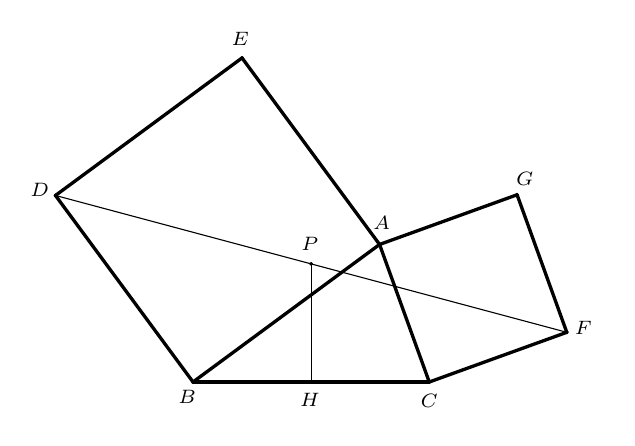
\begin{tikzpicture}[line cap=round,line join=round,>=triangle 45,x=1.5cm,y=1.5cm]
			\clip(-1.4,-0.3) rectangle (3.5,3.);
			\draw [line width=1.2pt] (0.,0.)-- (2.,0.);
			\draw [line width=1.2pt] (2.,0.)-- (1.5792841599472298,1.164470683441256);
			\draw [line width=1.2pt] (1.5792841599472298,1.164470683441256)-- (0.,0.);
			\draw [line width=0.4pt] (-1.1644706834412557,1.57928415994723)-- (3.1644706834412553,0.4207158400527701);
			\draw [line width=1.2pt] (2.,0.)-- (3.1644706834412553,0.4207158400527701);
			\draw [line width=1.2pt] (3.1644706834412553,0.4207158400527701)-- (2.7437548433884857,1.5851865234940257);
			\draw [line width=1.2pt] (2.7437548433884857,1.5851865234940257)-- (1.5792841599472298,1.164470683441256);
			\draw [line width=1.2pt] (1.5792841599472298,1.164470683441256)-- (0.4148134765059743,2.7437548433884853);
			\draw [line width=1.2pt] (0.4148134765059743,2.7437548433884853)-- (-1.1644706834412557,1.57928415994723);
			\draw [line width=1.2pt] (-1.1644706834412557,1.57928415994723)-- (0.,0.);
			\draw [line width=0.4pt] (1.,1.)-- (1.,0.);
			\begin{scriptsize}
				\draw [fill=black] (0.,0.) circle (0.5pt);
				\draw[color=black] (-0.04828924458152451,-0.12402492847733526) node {$B$};
				\draw [fill=black] (2.,0.) circle (0.5pt);
				\draw[color=black] (2.0002083162908733,-0.1567634739707296) node {$C$};
				\draw [fill=black] (1.5792841599472298,1.164470683441256) circle (0.5pt);
				\draw[color=black] (1.5979919002291696,1.3492096187254101) node {$A$};
				\draw [fill=black] (3.1644706834412553,0.4207158400527701) circle (0.5pt);
				\draw[color=black] (3.305073200956168,0.455915020262793) node {$F$};
				\draw [fill=black] (2.7437548433884857,1.5851865234940257) circle (0.5pt);
				\draw[color=black] (2.8093180834847655,1.7233644243642026) node {$G$};
				\draw [fill=black] (0.4148134765059743,2.7437548433884853) circle (0.5pt);
				\draw[color=black] (0.4006965221850284,2.9066289971968833) node {$E$};
				\draw [fill=black] (-1.1644706834412557,1.57928415994723) circle (0.5pt);
				\draw[color=black] (-1.2970309084009997,1.6298257229545041) node {$D$};
				\draw [fill=black] (1.,1.) circle (0.5pt);
				\draw[color=black] (0.989990341066129,1.1714860860469836) node {$P$};
				\draw [fill=black] (1.,0.) circle (0.5pt);
				\draw[color=black] (0.989990341066129,-0.1474096038297598) node {$H$};
			\end{scriptsize}
		\end{tikzpicture}
	\end{figure}
	\newpage
	\item 如图, 已知正方形$ABCD$的边长为$6$, $M$为$CD$上的一点. 连接$AM$并延长, 分别交$BD$, $BC$或其延长线于$E$, $F$. 过点$C$作$CG\perp CE$于$G$. 
	\begin{enumerate}[(1) ]
		\item 求证: $\angle DAE=\angle DCE$; 
		\item 当$M$为$CD$中点时, 若$P$, $Q$分别为$BC$, $BD$上的点, 求$\triangle MPQ$周长的最小值;
		\item 求$\sfrac{CG}{FM}$;
		\item 如图\textcircled{2}, 在(2)的条件下, 将$\triangle ADM$沿$AM$翻折得到$\triangle AHM$, 求$\tan\angle HAB$.
		\begin{figure}[H]
			\flushright
			\begin{minipage}{0.7\textwidth}
				\centering
				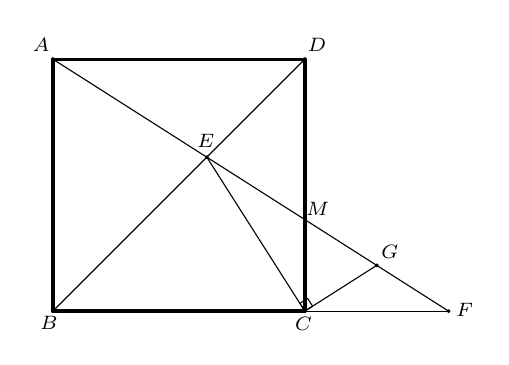
\begin{tikzpicture}[line cap=round,line join=round,>=triangle 45,x=0.8cm,y=0.8cm]
				\clip(-0.4,-0.4) rectangle (6.8,4.5);
				\draw[line width=0.4pt] (4.1231364082597235,0.0783988728789212) -- (4.044737535380802,0.2015352811386444) -- (3.921601127121079,0.12313640825972323) -- (4.,0.) -- cycle; 
				\draw [line width=1.2pt] (0.,4.)-- (0.,0.);
				\draw [line width=1.2pt] (0.,0.)-- (4.,0.);
				\draw [line width=1.2pt] (4.,0.)-- (4.,4.);
				\draw [line width=1.2pt] (4.,4.)-- (0.,4.);
				\draw [line width=0.4pt] (0.,0.)-- (4.,4.);
				\draw [line width=0.4pt] (6.282560130674044,0.)-- (4.,0.);
				\draw [line width=0.4pt] (2.4439672808457322,2.443967280845732)-- (4.,0.);
				\draw [line width=0.4pt] (4.,0.)-- (5.141280065337022,0.7266337554111568);
				\draw [line width=0.4pt] (0.,4.)-- (6.282560130674044,0.);
				\begin{scriptsize}
					\draw [fill=black] (0.,0.) circle (0.5pt);
					\draw[color=black] (-0.06180952026440939,-0.19246983666592257) node {$B$};
					\draw [fill=black] (4.,0.) circle (0.5pt);
					\draw[color=black] (3.977554141160235,-0.20623257486498428) node {$C$};
					\draw [fill=black] (4.,4.) circle (0.5pt);
					\draw[color=black] (4.190876583245694,4.232250494332423) node {$D$};
					\draw [fill=black] (0.,4.) circle (0.5pt);
					\draw[color=black] (-0.18567416405596576,4.232250494332423) node {$A$};
					\draw [fill=black] (2.4439672808457322,2.443967280845732) circle (0.5pt);
					\draw[color=black] (2.42924609376578,2.69770518513704) node {$E$};
					\draw [fill=black] (6.282560130674044,0.) circle (0.5pt);
					\draw[color=black] (6.537423446185734,0.020852605419534175) node {$F$};
					\draw [fill=black] (5.141280065337022,0.7266337554111568) circle (0.5pt);
					\draw[color=black] (5.346946591966886,0.936074695657139) node {$G$};
					\draw [fill=black] (4.,1.4532675108223139) circle (0.5pt);
					\draw[color=black] (4.2046393214447555,1.6173302365106943) node {$M$};
				\end{scriptsize}
			\end{tikzpicture}
				\caption*{\kaishu 图\textcircled{1}}
			\end{minipage}
					
			\begin{minipage}{0.7\textwidth}
				\centering
				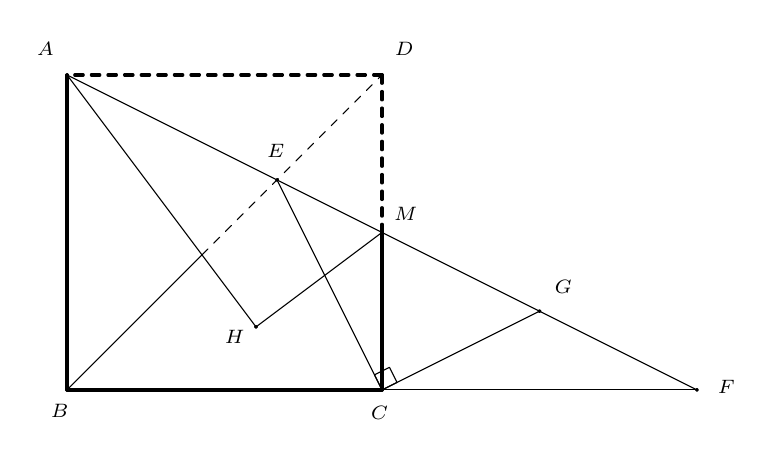
\begin{tikzpicture}[line cap=round,line join=round,>=triangle 45,x=1.0cm,y=1.0cm]
				\clip(-0.5,-0.6) rectangle (8.6,4.6);
				\draw[line width=0.4pt] (4.190834635391553,0.09541731769577688) -- (4.095417317695777,0.2862519530873306) -- (3.9045826823042233,0.1908346353915537) -- (4.,0.) -- cycle; 
				\draw [line width=1.2pt] (0.,4.)-- (0.,0.);
				\draw [line width=1.2pt] (0.,0.)-- (4.,0.);
				\draw [line width=1.2pt,dash pattern=on 3pt off 3pt] (4.,4.)-- (0.,4.);
				\draw [line width=0.4pt] (8.,0.)-- (4.,0.);
				\draw [line width=0.4pt] (2.6666666666666665,2.6666666666666665)-- (4.,0.);
				\draw [line width=0.4pt] (4.,0.)-- (6.,1.);
				\draw [line width=0.4pt] (0.,4.)-- (8.,0.);
				\draw [line width=0.4pt] (0.,4.)-- (2.4,0.8);
				\draw [line width=0.4pt] (2.4,0.8)-- (4.,2.);
				\draw [line width=0.4pt] (0.,0.)-- (1.7142857142857149,1.7142857142857146);
				\draw [line width=0.4pt,dash pattern=on 3pt off 3pt] (1.7142857142857149,1.7142857142857146)-- (4.,4.);
				\draw [line width=1.2pt,dash pattern=on 3pt off 3pt] (4.,4.)-- (4.,2.);
				\draw [line width=1.2pt] (4.,2.)-- (4.,0.);
				\begin{scriptsize}
					\draw [fill=black] (0.,0.) circle (0.5pt);
					\draw[color=black] (-0.09435980906923691,-0.2719168393351874) node {$B$};
					\draw [fill=black] (4.,0.) circle (0.5pt);
					\draw[color=black] (3.969019026450358,-0.29203257614469014) node {$C$};
					\draw [fill=black] (4.,4.) circle (0.5pt);
					\draw[color=black] (4.280812946997654,4.334586890040951) node {$D$};
					\draw [fill=black] (0.,4.) circle (0.5pt);
					\draw[color=black] (-0.2754014403547634,4.334586890040951) node {$A$};
					\draw [fill=black] (2.6666666666666665,2.6666666666666665) circle (0.5pt);
					\draw[color=black] (2.651438265427915,3.0371218658280212) node {$E$};
					\draw [fill=black] (8.,0.) circle (0.5pt);
					\draw[color=black] (8.374365387731505,0.03987708121210587) node {$F$};
					\draw [fill=black] (6.,1.) circle (0.5pt);
					\draw[color=black] (6.3024444963527,1.3071685002107816) node {$G$};
					\draw [fill=black] (4.,2.) circle (0.5pt);
					\draw[color=black] (4.3009286838071565,2.23249239344791) node {$M$};
					\draw [fill=black] (2.4,0.8) circle (0.5pt);
					\draw[color=black] (2.1284291083808387,0.6735227907114438) node {$H$};
				\end{scriptsize}
			\end{tikzpicture}
			\caption*{\kaishu 图\textcircled{2}}
			\end{minipage}
		\end{figure}
	\end{enumerate}
\end{enumerate}
\end{document}
